\chapter{Modelling Framework and Configuration}

\section{Python for Power System Analysis}
The PyPSA (Python for Power System Analysis) modelling framework is an open-source tool designed for simulating and optimizing modern power systems. It is capable of handling both steady-state and quasi-static time series simulations for systems that include features such as conventional generators, variable renewable energy, storage units, and more. The framework is particularly adept at facilitating the long-term investment planning needed for transitioning to renewable energy sources, thereby supporting the development of sustainable and cost-effective energy systems.


\section{Python for Power System Analysis-Europe}

%%%%
\subsection{Introduction to the Model}

PyPSA-Eur is an extension of the PyPSA framework, specifically designed to model the complexities of the European power system with openly available data. It optimises and models the European transmission network, encompassing the ENTSO-E area. The model includes components such as AC lines of 220 kV and above, substations, and HVDC links, facilitating cross-border electricity exchange and regional stability. The model's adaptability makes it valuable in various research contexts, from assessing policy impacts to exploring renewable energy expansion scenarios. \\

A key feature of PyPSA-Eur is its commitment to using only open and freely available data, enhancing its analyses' transparency and reproducibility. It is suitable for short-term operational and long-term infrastructure development planning studies.

%%%%%
\subsection{Long-Term Investment Planning}

Long-term investment planning in the energy sector is essential for developing a cost-effective, reliable, and sustainable future energy system. This process, extending over decades, must navigate uncertainties in technological advancements, policy shifts, market dynamics, and fluctuating energy demands. 

Within the PyPSA-Eur framework, energy system optimisation supports these long-term decisions. The model balances data inputs and constraints to identify an optimal system configuration. Its primary goal is minimising total system costs, considering new infrastructure investment and operational costs.\\

Long-term investment planning aims to minimise these total system costs over a set period, encompassing infrastructure capital costs and the marginal costs of energy production. The aim is to find an efficient mix of generation, storage, and transmission capacities that meet projected demand while adhering to constraints like system reliability, environmental regulations, and market conditions. The objective function is:

\begin{equation}
\begin{aligned}
\min \left[ \begin{array}{c}
\textbf{\textcolor{blue}{Annual}} \\
\textbf{\textcolor{blue}{System Costs}}
\end{array} \right] 
= \min \left[ \sum_{n} \left( \begin{array}{c}
\textbf{\textcolor{red}{Capital}} \\
\textbf{\textcolor{red}{Costs}}
\end{array} \right) + \sum_{n,t} \left( \begin{array}{c}
\textbf{\textcolor{teal}{Marginal}} \\
\textbf{\textcolor{teal}{Costs}}
\end{array} \right) \right]
\end{aligned}
\end{equation}

Here, \( n \) indexes network nodes representing different regions or sectors, and \( t \) denotes discrete time intervals, reflecting demand and supply variability.\\

PyPSA considers several critical factors for accurate optimisation. These include meeting energy demand at each node and time step, adhering to transmission constraints, and incorporating the variability of renewable sources like wind and solar. The model also considers geographical potentials for renewables, setting realistic limits on their expansion, and integrates environmental considerations, such as CO2 emission reduction targets. Furthermore, the model includes flexibility elements such as gas turbines, battery and hydrogen storage, and HVDC links.


\subsection{The Workflow} 
The PyPSA-Eur model features a structured workflow for modelling and optimizing complex energy systems to convert extensive datasets into actionable energy system planning and policymaking insights. The process begins with preparing the power system network, a critical step involving integrating spatial and temporal data, including infrastructure details, generation capacities, demand patterns, and renewable energy profiles.\\

Following establishing the initial network, the workflow moves into a simplification phase. This step, essential for making large-scale computations practical, involves strategies like network clustering and temporal data granulation reduction, maintaining computational efficiency while preserving the system's key dynamics.\\

The next stage is optimization, where PyPSA-Eur applies mathematical algorithms to identify the most efficient configuration of energy resources and transmission infrastructure. This stage balances operational costs with long-term infrastructure investments, addressing operational and investment decisions.\\

The final step involves summarizing and interpreting the results. This phase analyzes the outcomes, focusing on various energy scenarios' cost-effectiveness, reliability, and sustainability. Stakeholders need to comprehend the modelling implications, serving as a foundation for informed decision-making.\\

\begin{figure}[H]
\centering
\includesvg[width=0.6\textwidth]{Figure/simplified_workflow.svg}
\caption{The PyPSA-Eur Workflow}
\label{fig:pypsa-workflow}
\end{figure}

Throughout this workflow, PyPSA-Eur emphasizes configure-ability and adaptability. It allows parameter adjustments such as country selection, temporal resolution, and cost assumptions to suit different analytical needs and scenarios.





\subsection{Preparing Networks}
In the PyPSA-Eur framework, preparing networks involves a series of configurable elements crucial to tailoring the model to specific analytical needs. The process starts with country selection, determining the geographic scope of the study and enabling the model to focus on either individual national grids or regional interconnected systems.\\

Setting the reference year or time period is another key element, allowing the model to address different temporal dynamics. This is vital for both retrospective analyses and future projections, informing strategies for energy system development and transition.\\

Integrating a CO2 budget aligns the model with environmental policy objectives, simulating the impact of varying climate policy stringencies on energy system optimization. This is essential for aligning the model with emission reduction targets.\\

Adjusting spatial and temporal resolution offers the flexibility to vary the detail level, enabling more nuanced local insights or broader strategic assessments. High-resolution settings are particularly useful for detailed local impact analysis, while lower resolutions are better suited for general strategic reviews.\\

Cost assumptions can be tailored to reflect current economic conditions and anticipated future developments. This flexibility is crucial for accurately simulating the economic feasibility of different energy technologies across varying scenarios.\\

Technology parameterization within the framework allows for an accurate representation of various energy sources and infrastructure, including their efficiency, capacity, operational lifespan, and maintenance needs.\\

Defining land use eligibility criteria addresses non-technical constraints on energy infrastructure deployment, ensuring that the model's recommendations are viable within real-world geographical and regulatory contexts.\\

Choosing an appropriate weather dataset is critical for accurately modeling the variability and availability of renewable energy sources, providing insight into the integration of weather-dependent resources like wind and solar power.\\

The option to focus on greenfield generation expansion or optimizing existing power plants provides the flexibility to explore new infrastructure possibilities or improve the efficiency and capacity of existing assets. This choice is fundamental in shaping the model's approach to energy system optimization.\\

Overall, network preparation in PyPSA-Eur is an extensive process, encompassing a wide range of factors, each adjustable to align the analyses with specific technical, economic, or policy objectives.\\

The PyPSA-Eur framework's adaptability is evident in its comprehensive array of configurable elements, essential for tailoring the model to various scenarios. Table 1 summarizes these elements, from geographical and temporal settings to economic and technological parameters, offering a clear guide for customizing the framework to specific energy analysis requirements.

\begin{table}[H]
\centering
\caption{Configurable Elements for PyPSA-Eur Analysis}
\label{tab:pypsa_config}
\renewcommand{\arraystretch}{1.5} % Adjust for spacing
\begin{tabular}{ll}
\textbf{Configurable Element} & \textbf{Description} \\
\midrule
Country Selection & Determines the model's geographic scope. \\
Reference Year / Time Period & Sets the temporal context for analysis. \\
CO2 Budget & Limits emissions for climate policy alignment. \\
Spatial and Temporal Resolution & Defines granularity in geographical and time dimensions. \\
Cost Assumptions & Tailors economic parameters to reflect market conditions. \\
Technology Parameterization & Details operational and physical characteristics of energy technologies. \\
Land Use Eligibility Criteria & Sets geographical constraints for infrastructure. \\
Weather Dataset Selection & Chooses meteorological data for renewable energy modeling. \\
Solver Selection & Selects the optimization algorithm for analysis. \\
Greenfield vs. Existing Power & Focuses on either new developments or existing infrastructure. \\
\end{tabular}
\end{table}





\subsection{Land Availability for Renewable Energy}
Land availability assessment for renewable energy installations is a crucial component of the PyPSA-Eur model, ensuring realistic and sustainable energy planning. The model utilizes the CORINE 2018 land cover dataset to identify suitable areas for renewable installations, particularly for onshore wind farms. This dataset's detailed classification of land cover types across Europe, such as agricultural land, forests, and urban areas, aids in determining viable locations for renewable energy infrastructure.\\

Moreover, PyPSA-Eur accounts for environmental conservation by integrating the NATURA 2000 natural protection areas into its analysis. These areas, designated for the preservation of endangered species and habitats, impose restrictions on the deployment of renewable energy infrastructure, ensuring compatibility with environmental conservation goals.\\

The GEBCO 2018 bathymetry dataset, crucial for offshore energy projects, is also incorporated. This dataset provides insights into underwater terrain, beneficial for planning offshore wind farms and assessing their potential environmental impacts.\\

A key aspect of the model's analysis is the density of renewable energy installations, expressed as capacity per square kilometer. This metric is vital in determining the potential energy yield from a given land area, factoring in technological capabilities and local geographic conditions. An example in the model illustrates estimating potential energy output from a single geographic cell, based on land availability and technology-specific parameters.\\

In assessing offshore wind farm potential in the Baltic Sea Region, PyPSA-Eur uses maps (images 24-29) to visualize eligible areas for development, taking into account environmental and technical constraints. These maps show the geographic potential for offshore wind energy, with areas like the Baltic Sea Region highlighted due to their dense wind resource concentration.\\

The maps also depict variations in potential across different regions, indicating where the highest energy generation per square kilometer might be achievable. This helps in identifying optimal locations for new installations. Environmental protection statuses and technical constraints are overlaid to identify eligible areas for development, balancing offshore wind energy expansion with environmental preservation goals.\\

Differentiating between AC and DC offshore wind potential, the maps inform on suitable areas for each transmission technology, crucial for planning, especially considering the specific needs of the Baltic Sea Region's isolated grids or long-distance transmission requirements.\\

These visual representations are integral to the PyPSA-Eur model, providing spatial data needed to simulate and optimize energy systems. In studies focusing on the Baltic Sea Region, these maps form the basis for scenario analysis of offshore wind development, guiding resource allocation and integration strategies for new wind farms into the European power grid. This visual data is thus key to strategic planning and policymaking, directing the sustainable growth of offshore wind energy in the Baltic Sea Region.

\begin{figure}[htp]
    \centering
    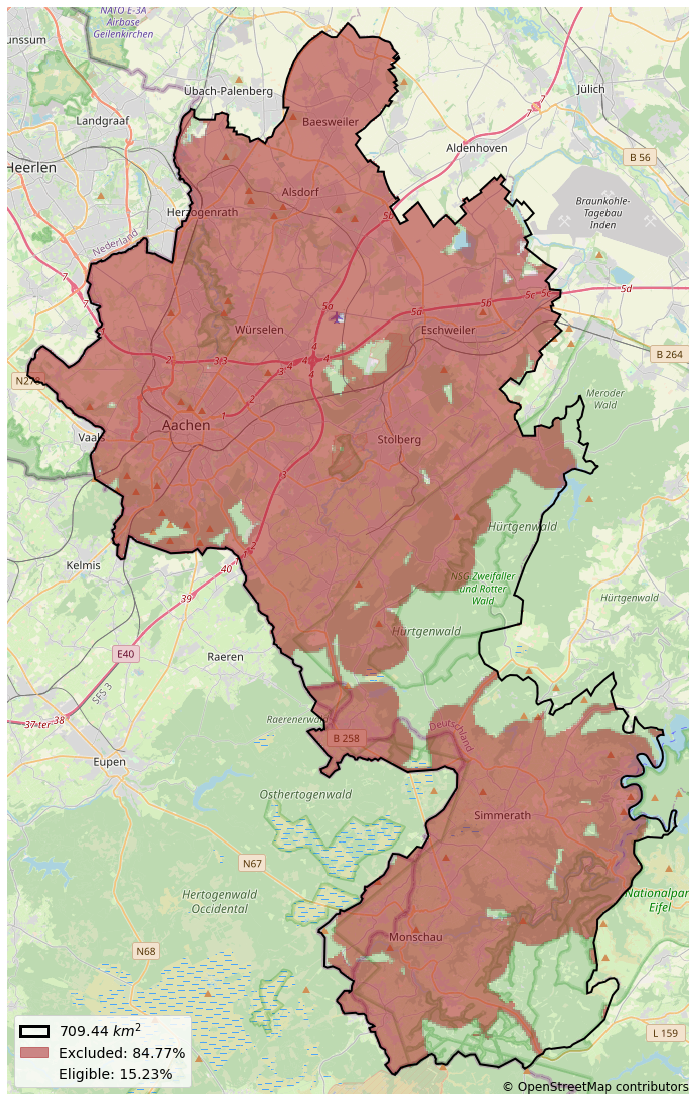
\includegraphics[width=0.45\textwidth]{Figure/land_availability.png}
    \caption{Land Availability}
    \label{fig:land_availability}
\end{figure}


\begin{figure}[htp]
    \centering
    % First row - Eligible Area
    \begin{subfigure}{0.45\textwidth}
        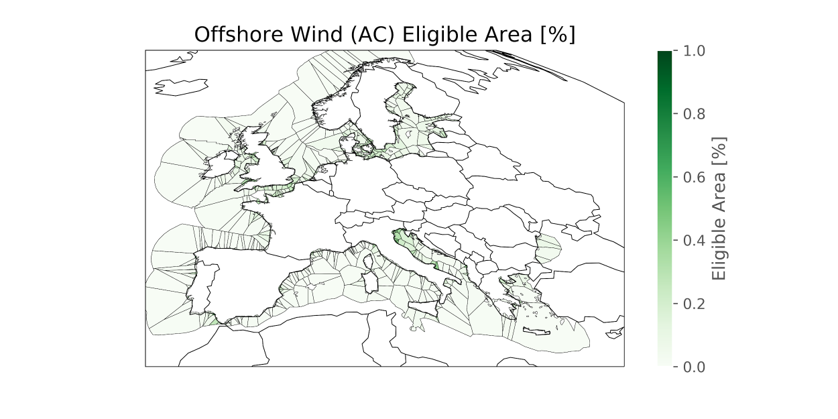
\includegraphics[width=\textwidth, trim=3.5cm 0cm 2.5cm 0cm, clip]{Figure/offshore_wind_AC_eligible_area_mesh.png}
        \caption{Offshore Wind (AC) Eligible Area}
    \end{subfigure}
    \hfill
    \begin{subfigure}{0.45\textwidth}
        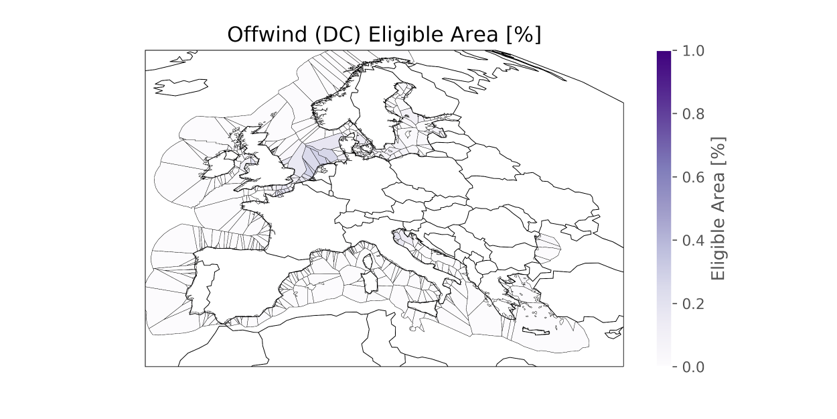
\includegraphics[width=\textwidth, trim=3.5cm 0cm 2.5cm 0cm, clip]{Figure/offshore_wind_DC_eligible_area_mesh.png}
        \caption{Offwind (DC) Eligible Area}
    \end{subfigure}
    
    % Second row - AC Geographic Potential
    \begin{subfigure}{0.45\textwidth}
        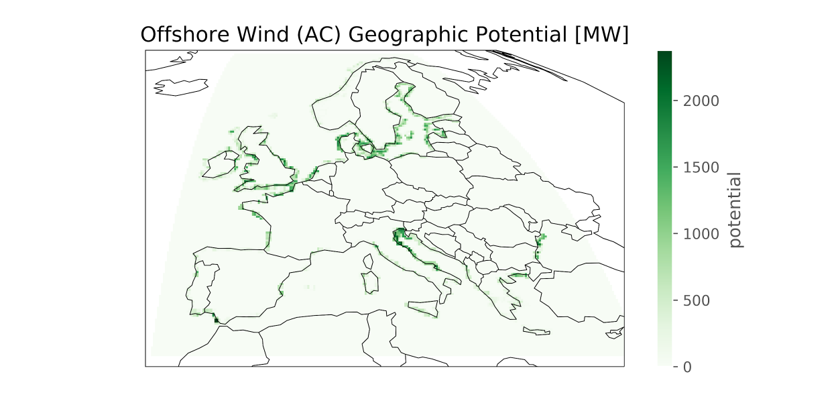
\includegraphics[width=\textwidth, trim=3.5cm 0cm 2.5cm 0cm, clip]{Figure/offshore_wind_AC_potential.png}
        \caption{Offshore Wind (AC) Geographic Potential}
    \end{subfigure}
    \hfill
    \begin{subfigure}{0.45\textwidth}
        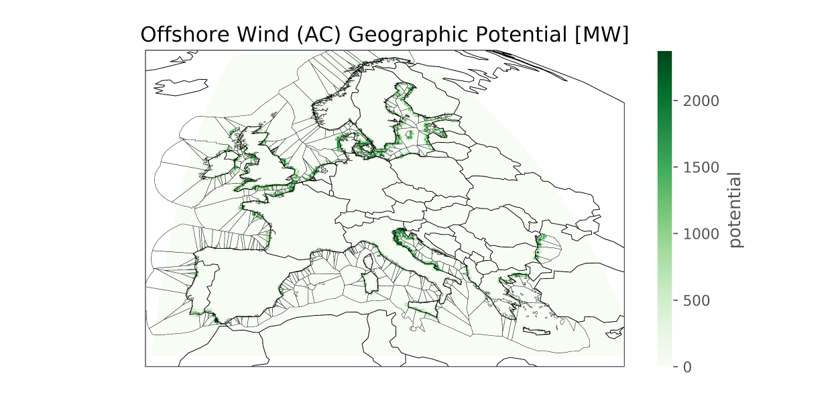
\includegraphics[width=\textwidth, trim=3.5cm 0cm 2.5cm 0cm, clip]{Figure/offshore_wind_AC_potential_mesh.png}
        \caption{Offshore Wind (AC) Potential Mesh}
    \end{subfigure}
    
    % Third row - DC Geographic Potential
    \begin{subfigure}{0.45\textwidth}
        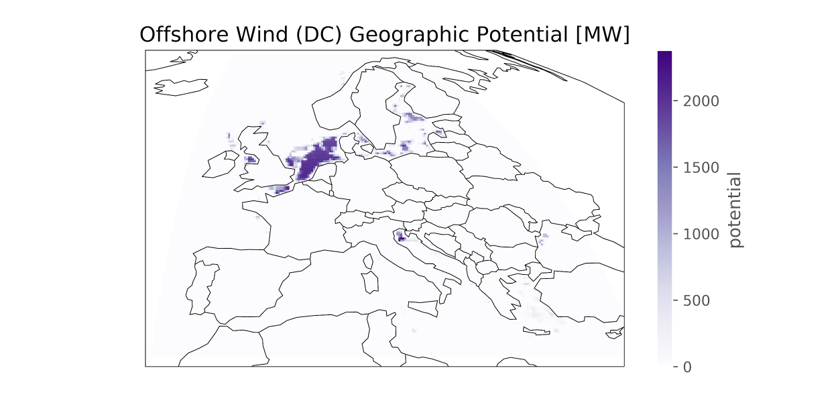
\includegraphics[width=\textwidth, trim=3.5cm 0cm 2.5cm 0cm, clip]{Figure/offshore_wind_DC_potential.png}
        \caption{Offshore Wind (DC) Geographic Potential}
    \end{subfigure}
    \hfill
    \begin{subfigure}{0.45\textwidth}
        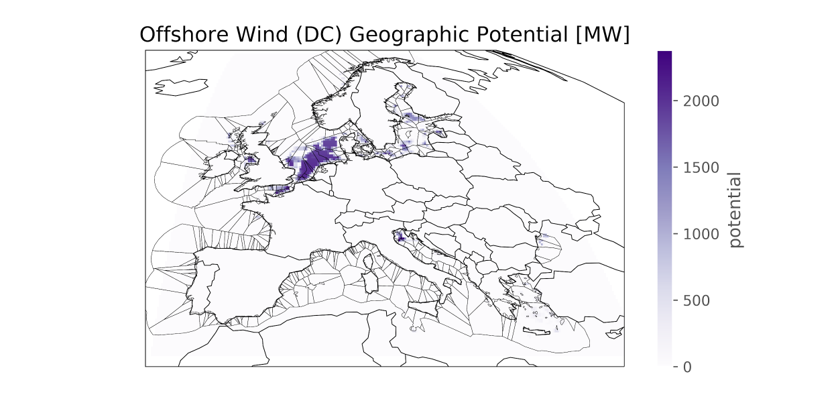
\includegraphics[width=\textwidth, trim=3.5cm 0cm 2.5cm 0cm, clip]{Figure/offshore_wind_DC_potential_mesh.png}
        \caption{Offshore Wind (DC) Potential Mesh}
    \end{subfigure}
    
    \caption{Comparison of eligible areas and geographic potential for Offshore Wind AC and DC}
\end{figure}







\subsection{Time Series for Renewable Energy}
Integrating time series for renewable energy is a critical aspect of the PyPSA-Eur model, especially for simulating and optimizing variable renewable sources like wind and solar power. These time series reflect the inherent intermittency and variability of renewable energy, influenced by meteorological and climatic factors, and are essential for the model's accuracy in representing renewable generation.\\

In PyPSA-Eur, renewable energy time series are sourced from comprehensive weather datasets such as ERA-5 and SARAH-2. These datasets provide up to 40 years of historical weather data at high spatial resolution, crucial for analyzing renewable energy patterns and forecasting generation potential. Wind time series, for example, capture fluctuations in wind speed and direction, which are vital for predicting wind turbine outputs. Solar time series account for variables like solar irradiance, incidence angle, and sunlight duration, impacting solar panel energy yields.\\

The model translates these weather variables into power generation estimates using detailed models of solar panels and wind turbines. Factors like solar panel orientation and material, as well as wind turbine power curves and surface roughness, are considered in converting meteorological data into expected energy output. This results in comprehensive time series representing potential electricity generation from renewables at various locations and times.\\

These time series are instrumental in energy system planning and operation, enabling the assessment of renewable supply against demand over time and across different weather scenarios. They are vital for designing systems that can handle renewable energy's production peaks and troughs, ensuring power supply reliability and stability. Additionally, the time series guide the scaling and selection of storage solutions and flexibility options to mitigate renewable energy variability.\\

\subsection{Simplifying Networks}
Network simplification in the PyPSA-Eur framework is a strategic measure to manage the computational demands of power system modeling. This simplification is crucial for the co-optimization of generation, storage, and transmission within an integrated energy system.\\

The process starts by standardizing transmission lines to a common voltage level, typically 380kV, and eliminating network redundancies. This reduces variables and simplifies analysis, allowing the model to concentrate on key transmission pathways.\\

Network clustering, using methods like k-means, further streamlines the model. This approach groups network nodes based on generation, demand, and location similarities, resulting in a simplified network that retains the original system's essential characteristics but with fewer nodes and lines, easing computational demands.\\

Subsequently, storage units and demand-side resources are incorporated into the simplified network. These components are key to modeling the system's operational flexibility and the potential of various energy storage and demand response strategies.\\

Finally, the simplification includes snapshot aggregation and the application of system-wide constraints. Snapshots, representing specific system states like demand and renewable generation, are consolidated into representative periods to reduce temporal complexity. System-wide constraints, such as emissions limits or renewable targets, ensure the model aligns with broader policy and sustainability objectives.\\

By simplifying networks, PyPSA-Eur maintains computational feasibility while providing insightful results, a crucial step for large-scale models guiding the transition to a sustainable and resilient energy system.


\subsection{Solving the Optimization Problem}
At the core of the PyPSA-Eur model is the optimization problem, focused on the strategic allocation of energy resources for a sustainable future power system. The goal is to minimize overall costs while adhering to constraints like energy demand, transmission capacity, and carbon emission targets. This complex balancing act necessitates advanced mathematical and computational techniques.\\

PyPSA-Eur utilizes linear programming (LP) or mixed-integer linear programming (MILP) for solving this problem. The choice between LP and MILP depends on the model's complexity and the presence of discrete decision variables. These optimization methods excel in managing large-scale systems with numerous variables and constraints, systematically exploring feasible solutions to find the most cost-effective configuration of generation, transmission, and storage within the given constraints.\\

The optimization considers various costs: capital expenditures for new infrastructure, operational and maintenance expenses, fuel prices, and potential electricity sale revenues. It also integrates the cost of carbon emissions to comply with climate policies. Different time periods, each with unique demand profiles and renewable energy availability, are factored in, utilizing the detailed time series data in the model.\\

For variable renewable sources like wind and solar, the optimization must account for their intermittency and unpredictability. The renewable energy time series are vital here, ensuring supply meets demand consistently.\\

Upon solving the optimization problem, PyPSA-Eur delineates the optimal system layout, detailing power plant locations, transmission line capacities and routes, and the scale and distribution of storage facilities. This configuration enables analysis of operational strategies and investment needs for an efficient, sustainable energy system.\\

Importantly, the optimization results from PyPSA-Eur offer practical insights for policymakers, energy planners, and industry stakeholders. They guide informed decisions on energy system development, playing a critical role in Europe's shift towards a low-carbon energy future. Through this rigorous optimization, PyPSA-Eur significantly contributes to the strategic planning needed for this transition.

\subsection{Summarizing the Results}
The culmination of the PyPSA-Eur modelling process lies in effectively summarizing its results. This crucial phase involves translating the complex outputs of the optimization into clear, actionable insights. The summary highlights the most cost-effective and efficient strategies for developing Europe's future energy system, identifying key areas for investment in generation, storage, and transmission.\\

This summary delineates the optimal energy mix and its evolution over the study period. It details how various energy sources meet demand, emphasizing the significant roles and locations for renewable energy integration. Stakeholders can glean insights into the geographical distribution of renewable potentials and how these align with environmental and policy constraints.\\

A critical component of the summary is its economic analysis. It itemizes the total system cost, breaking it down into capital expenditure, operational expenses, and potential savings from emission reductions and efficiency improvements. This economic breakdown is fundamental for evaluating the transition's feasibility and sustainability, offering a comprehensive view of its long-term financial implications.\\

In terms of policy guidance, the summary offers strategies for meeting emission targets and integrating renewables while ensuring system reliability. It provides valuable input for policymaking on subsidies, tariffs, and investments, aligning them with the model's insights.\\

Moreover, the summary serves as a bridge between the model's technical data and the practical aspects of implementing the future energy system. It translates complex technical details into an accessible narrative, aiding public understanding and informed decision-making.\\

Overall, the PyPSA-Eur results provide a comprehensive view of the multifaceted aspects of energy system planning, offering a clear guide to addressing the challenges and seizing the opportunities in Europe's journey towards a resilient, sustainable, and cost-effective energy future.

\section{Python for Power System Analysis-North Sea}






